\begin{figure}[!htbp]\centering
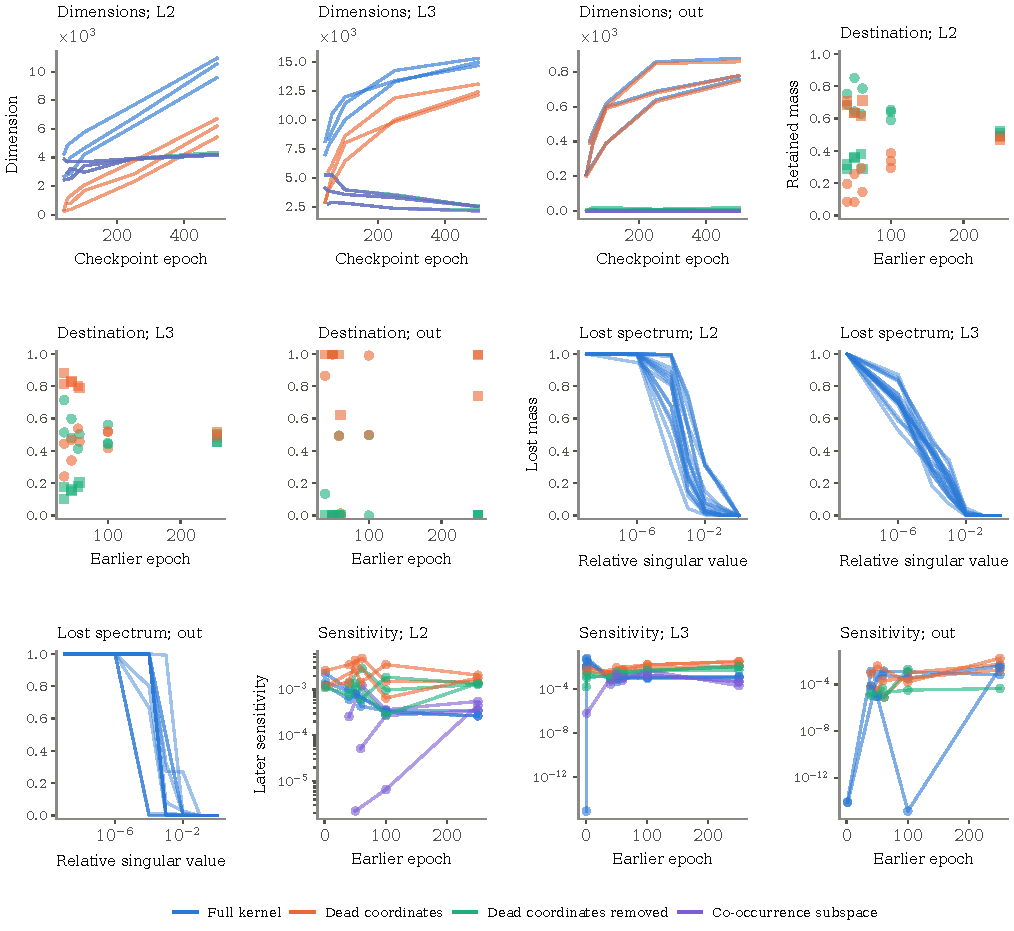
\includegraphics[width=6.081in]{persistence_diagnostics.pdf}
\caption{Further ReLU persistence diagnostics, all measured layers, pairs and three seeds. Panels 1--3: dimensions of the full kernel and its component spaces. Panels 4--6: the earlier kernel with dead coordinates removed, split into mass retained in later non-dead directions (green) and later dead coordinates (orange); circles denote consecutive pairs and squares comparisons ending at epoch 500. Panels 7--9: cumulative lost mass carried by later singular directions above each relative singular-value threshold. Panels 10--12: median later sensitivity of 32 sampled directions from the earlier kernel (blue) and its positive tails at thresholds $10^{-3}$ (orange), $10^{-4}$ (green) and $10^{-6}$ (purple). Missing curves denote empty or unresolved spaces.}\label{fig:persistence-diagnostics}
\end{figure}
\begin{table}[!htbp]\centering
\caption{GELU numerical dead-coordinate sensitivity at epoch 500, width 128. A unit is counted when its derivative magnitude is at most $\tau$ on every analysis image. Coordinate dimensions are seed ranges. The last columns count seeds whose dead-coordinate and co-occurrence projector splits resolve, out of three. The co-occurrence split remains unresolved at the endpoint.}\label{tab:persistence-gelu-tau}
\small\begin{tabular}{llrrr}\toprule
Layer & $\tau$ & Coordinate dimension & Dead split & Deficit split\\\midrule
2 & $10^{-9}$ & 258--774 & 3/3 & 0/3\\
3 & $10^{-9}$ & 256--768 & 3/3 & 0/3\\
2 & $10^{-6}$ & 774--1806 & 0/3 & 0/3\\
3 & $10^{-6}$ & 768--1792 & 1/3 & 0/3\\
2 & $10^{-3}$ & 2064--3096 & 0/3 & 0/3\\
3 & $10^{-3}$ & 2624--3282 & 0/3 & 0/3\\
\bottomrule\end{tabular}\end{table}\FloatBarrier
